\section{压力和压强}\label{sec:5-1}

人站在松软的地上,会在地面上压出深深的脚印。
这是因为人受重力作用,站在地面上时就压着地面,对地面有一个向下的作用力。
用力往墙上按图钉,图钉就钉进墙里,这是因为手按图钉时,钉尖就压着墙面,
对墙面有一个作用力(图 \ref{fig:5-1})。上面例子中的地面、墙面受到的力都是跟它们的表面垂直的,
我们把这种\textbf{垂直作用在物体表面上的力叫做压力}。房屋对地基、汽车对路面都产生压力。
用手握住物体,用钳子夹住物体,手和钳子对物体也产生压力。

用同样的力往墙上按图钉,尖的图钉容易按进去,钝头的图钉就很难按进去,这是为什么呢?
下面我们来研究这个问题。

\begin{figure}[htbp]
    \centering
    \begin{minipage}{6cm}
    \centering
    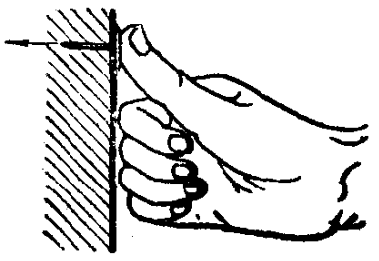
\includegraphics[width=4cm]{../pic/czwl1-ch5-1}
    \caption{}\label{fig:5-1}
    \end{minipage}
    \qquad
    \begin{minipage}{8cm}
    \centering
    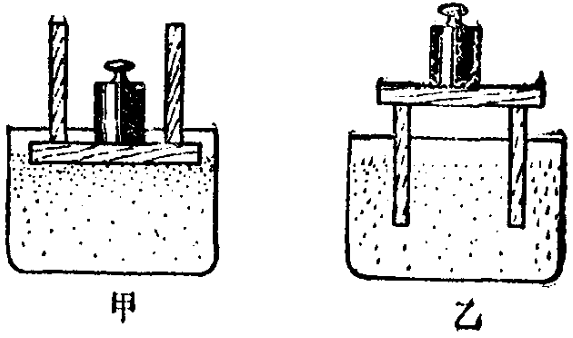
\includegraphics[width=6cm]{../pic/czwl1-ch5-2}
    \caption{}\label{fig:5-2}
    \end{minipage}
\end{figure}


我们先做一个实验。取一个有四条腿的小木桌,先把桌面放在沙上(图 \ref{fig:5-2} 甲),往桌面上放重物,
可以看到,放的重物越重,桌面陷进沙里越深。
把小桌翻过来让桌腿立在沙上(图 \ref{fig:5-2} 乙),再把同样的重物放在桌上,可以看到,桌腿陷进沙里更深了。

为什么同样的重物在两种情况下产生的效果不同呢?
这是因为桌面放在沙上时,压力作用在桌面那么大的面积上;
桌腿放在沙上时,压力只作用在四条桌腿那么大的面积上,而四条桌腿的面积比桌面的面积要小得多。

同样的道理可以说明按图钉的问题。因为尖的图钉比钝头的图钉面积小,所以容易按进墙里去。

\begin{figure}[htbp]
    \centering
    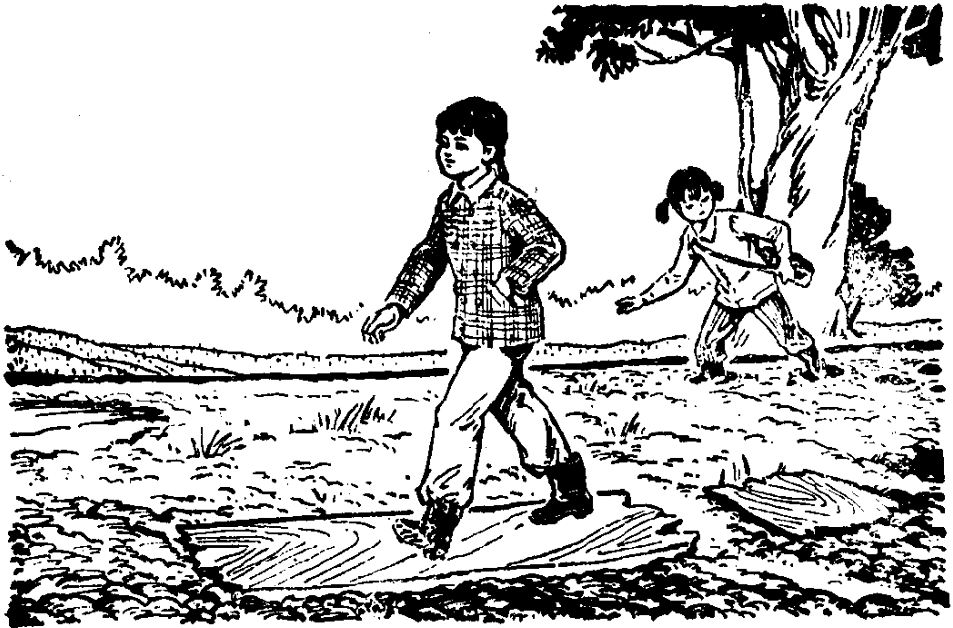
\includegraphics[width=0.6\textwidth]{../pic/czwl1-ch5-3}
    \caption{}\label{fig:5-3}
\end{figure}

我们再分析一个例子。人在烂泥地上走,脚会深深地陷进泥里,如果在烂泥地上垫一块木板,就不会陷下去了(图 \ref{fig:5-3})。
这是因为没有垫木板时,压力是作用在脚掌那么大的面积上,垫了木板以后,压力就作用在木板那么大的面积上了。

可见\CJKunderwave{压力产生的效果不仅跟压力的大小有关系,而且跟受力面积的大小也有关系}。
压力越大,效果越明显;受力面积越小,效果越明显。

既然压力产生的效果跟压力的大小和受力的面积都有关系。
那么为了比较压力的效果,就要取相同的面积上受到的压力来进行比较。
一般总是取单位面积上受到的压力来进行比较的。
我们把\textbf{物体的单位面积上受到的压力叫做压强}。

在国际单位制中,力的单位是牛顿,面积的单位是平方米,
所以就取 1 平方米面积上受到的压力作为压强。
如果作用在 $4 \pfm$ 面积上的压力是 600 牛顿,那么压强就是
$$ \dfrac{600 \text{牛顿}}{4 \pfm} = 150 \ndmpfm \juhao $$

因此计算压强的公式是
$$ \text{压强} = \dfrac{\text{压力}}{\text{面积}} \; \juhao $$

如果用 $p$ 表示压,$F$ 表示压力,$S$ 表示受力面积,那么上面的压强公式可以写成
$$ p = \dfrac{F}{S} \; \juhao $$

从上面的计算可以看出,压强单位是“$\ndmpfm$”,读作“牛顿每平方米”,意思是每平方米面积上的压力是多少牛顿。
$\ndmpfm$ 有一个专门的名称叫做\textbf{帕斯卡},这是为了纪念法国科学家帕斯卡。
$$ 1 \pasika = 1 \ndmpfm \;\juhao $$

帕斯卡是一个很小的压强单位。一粒西瓜子平放时对桌面的压强大约是 20 帕斯卡。
一块砖平放时对地面的压强有 1000 多帕斯卡。

\liti 一个质量是 60 千克的人,他每只脚接触地面的面积是 $170 \pflm$,这个人站立时对地面的压强是多大?

人站立时是两只脚接触地面的。地面受到的压力等于人受到的重力。

解:地面受到的压力
$$ F = G = mg = 60 \text{千克} \times 9.8 \text{牛顿/千克} = 588 \niudun \;\juhao $$

地面的受力面积
$$ S = 170 \pflm \times 2 = 340 \pflm = 0.034 \pfm \;\juhao $$

地面受到的压强
$$ p = \dfrac{F}{S} = \dfrac{588 \niudun}{0.034 \pfm} \approx 17\; 000 \ndmpfm = 1.7 \times 10^4 \pasika \;\juhao $$

答:人对地面的压强是 $1.7 \times 10^4 \pasika$。

有兴趣的同学,可以测量一下自己的体重和鞋底的面积,算算你站立时对地面的压强大约是多大。


